\documentclass[a4paper, 11pt]{article}
\usepackage{covington}
\usepackage{amssymb}
\usepackage{amsmath}
\usepackage[catalan]{babel}
\usepackage{graphicx}
\usepackage{eurosym}
\textheight=23.94cm 
\textwidth=17cm 
\topmargin=-1cm 
\oddsidemargin=-0.5cm 
 
\newcommand{\header}[4]{
	\begin{center}
		\rule{\linewidth}{0.5pt}
		
		{\small{#1}}
      
        \vspace{0.2in}
        
		{\large{#2}}
		
        \vspace{0.2in}
        
		{\small{#3}}
		
		\vspace{0.15in}
		
		{#4}
		
		\vspace{-0.1in}
		\rule{\linewidth}{0.6pt}
	\end{center}
}

\usepackage{Sweave}
\begin{document}
\Sconcordance{concordance:ps2_v5.tex:ps2_v5.Rnw:%
1 35 1 1 0 35 1 1 30 32 0 1 2 1 22 24 0 1 2 8 1 1 30 32 0 1 2 59 1}

 
\header{\sc Barcelona Graduate School of Economics \hfill Master's Degree in Data Science}{\bf Statistical Modeling and Inference $-$ Problem Set \#2}{\sc Niti Mishra $\cdot$ Miquel Torrens $\cdot$ B\'alint V\'an}{October 18\textsuperscript{th}, 2015}
Solution to proposed exercises.\\
% PROBLEM SET 2 (PART 1)
% EXERCISE 1
\newline \textbf{\underline{Exercise 1}}\\
\newline We need to solve:
\begin{eqnarray}
\max_{\mathbf{w}} -2 \log p(\mathbf{w | t, X}) &=&  -2q \mathbf{t}^T \mathbf{\Phi w} + q \mathbf{w}^T \mathbf{\Phi}^T \mathbf{\Phi w} + (\mathbf{w - \mu})^T \mathbf{D} (\mathbf{w - \mu}) + C \nonumber \\
&=&  -2q \mathbf{t}^T \mathbf{\Phi w} + q \mathbf{w}^T \mathbf{\Phi}^T \mathbf{\Phi w} + \mathbf{w}^T \mathbf{D w} - 2 \mathbf{w}^T \mathbf{D} \mathbf{\mu} + \mathbf{\mu}^T \mathbf{D \mu} + C \nonumber
\end{eqnarray}
The term $C$ includes all constant terms not dependant on $\mathbf{w}$. Now we maximize with respect to $\mathbf{w}$ and set to zero:
\begin{eqnarray}
-2q \mathbf{t}^T \mathbf{\Phi} + q \mathbf{w}^T \left(\mathbf{\Phi}^T \mathbf{\Phi} + \left( \mathbf{\Phi}^T \mathbf{\Phi} \right)^T \right) + \mathbf{w}^T \left( \mathbf{D} + \mathbf{D}^T \right) - 2 \left( \mathbf{D} \mathbf{\mu} \right)^T = 0 \nonumber
\end{eqnarray}
During the derivation we will recurrently use two properties: $\mathbf{D} = \mathbf{D}^T$, as it is symmetric by construction, and $\left( \mathbf{\Phi}^T \mathbf{\Phi} \right)^T = \mathbf{\Phi}^T \mathbf{\Phi}$, which is a straightforward calculation. We just need to rearrange terms to reach the normal equations:
\begin{eqnarray}
2 \mathbf{w}^T\mathbf{D} -2 \mathbf{\mu}^T \mathbf{D}^T -2 q \mathbf{t}^T \mathbf{\Phi} + 2q\mathbf{w}^T \mathbf{\Phi}^T \mathbf{\Phi} &=& 0 \nonumber \\
\mathbf{w}^T \left( \mathbf{D} + q \mathbf{\Phi}^T \mathbf{\Phi} \right) &=& q\mathbf{t}^T \mathbf{\Phi} + \left( \mathbf{D\mu} \right)^T  \nonumber \\
\left( \mathbf{D} + q \mathbf{\Phi}^T \mathbf{\Phi} \right)^T \mathbf{w} &=& q\mathbf{\Phi}^T \mathbf{t} + \left( \mathbf{D\mu} \right) \nonumber
\end{eqnarray}
To finally obtain the normal equations:
\begin{eqnarray}
\left( \mathbf{D} + q \mathbf{\Phi}^T \mathbf{\Phi} \right) \mathbf{w} = q\mathbf{\Phi}^T \mathbf{t} + \mathbf{D\mu} \nonumber
\end{eqnarray}
Hence proved.\\
% EXERCISE 2
\newpage
\textbf{\underline{Exercise 2}}\\
\newline \underline{Part 1}. Plotting the data:\\
\begin{center}
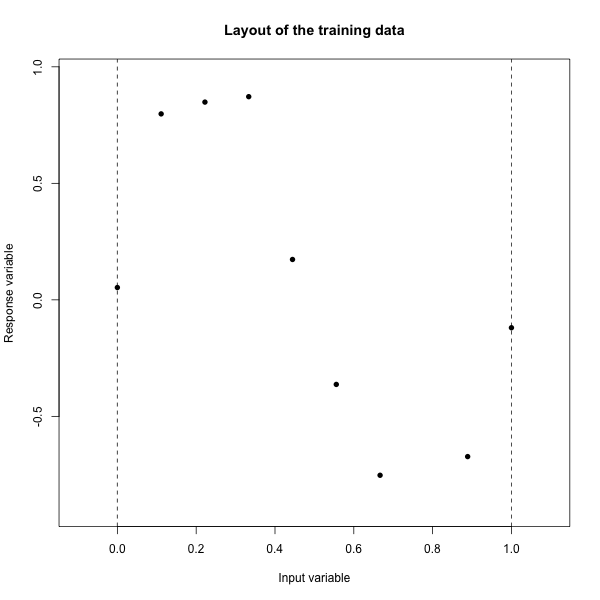
\includegraphics[scale=0.6]{ps2_plot1.png}
\end{center}
\underline{Part 2}. The \texttt{phix} function:
\begin{Schunk}
\begin{Sinput}
> ################################################################################
> # Function "phix"
> phix <- function(x, M, basis) {
+ ################################################################################
+   # Check correctness of input x
+   if (x < 0 || x > 1) {
+     stop('out-of-range values in the input vector "x".')
+   }
+   
+   # Perform the calculations  
+   if (basis == 'poly') {
+     out <- rep(NA, length = M + 1)
+     sapply(c(0, 1:M), function(i) {
+       out[i + 1] <<- x^i
+     })
+   } else if (basis == 'Gauss') {
+     mus <- seq(0, 1, length.out = M)
+     out <- rep(NA, length = M)
+     sapply(1:M, function(i) {
+       out[i] <<- exp((-(x - mus[i]) ** 2) / 0.1)
+     })
+     out <- c(1, out)
+   } else {
+     stop('specify a valid option for the parameter "basis".')
+   }
+   
+   # Return the values
+   return(out)
+ }
\end{Sinput}
\end{Schunk}
\underline{Part 3}. The \texttt{post.params} function:
\begin{Schunk}
\begin{Sinput}
> ################################################################################
> # Function "post.params"
> post.params <- function(tdata, M, basis, phix, delta, q) {
+ ################################################################################
+   # Input data
+   t <- tdata[, 't']  # Response variable
+   x <- tdata[, 'x']  # Input variable
+   
+   # Initialize Phi matrix
+   phi <- matrix(nrow = length(x), ncol = M + 1)
+   sapply(1:length(x), function(i) {
+     phi[i, ] <<- phix(x = x[i], M = M, basis = basis)
+   })
+ 
+   # Parameter estimation
+   Q <- delta * diag(ncol(phi)) + q * t(phi) %*% phi
+   w.bayes <- q * solve(Q) %*% t(phi) %*% t
+     
+   # Results
+   return(list(w.bayes = w.bayes, Q = Q))
+ }
\end{Sinput}
\end{Schunk}
\underline{Part 4}. Plotting the estimated linear predictor:
\begin{center}
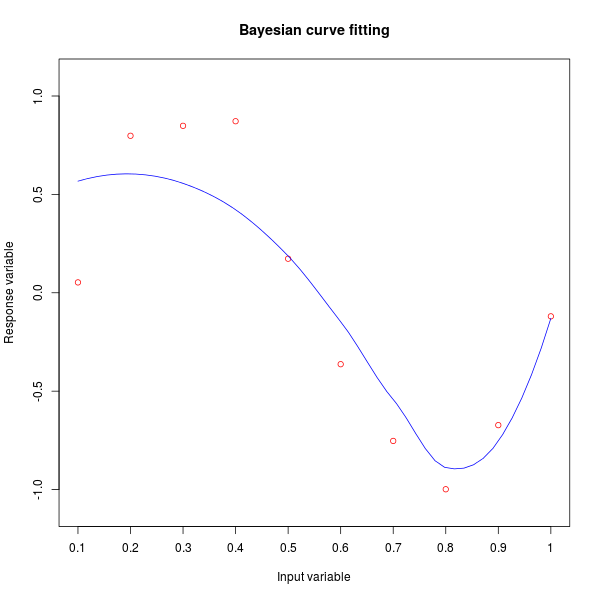
\includegraphics[scale = 0.5]{ps2_plot2.png}
\end{center}
% PROBLEM SET 2 (PART 2)
% EXERCISE 3
\newpage
\textbf{\underline{Exercise 3}}\\
\newline \underline{Part 1}. The function that returns the mean and the precision of the predictive distribution at each of the inputs:
\begin{Schunk}
\begin{Sinput}
> ################################################################################
> bayesian.precision <- function(x) {
+ ################################################################################
+   # Parameters
+   M <- 9
+   delta <- 1L
+   q <- 0.1 ** (-2)
+   
+   # Initialize Phi matrix
+   phi <- matrix(nrow = length(x), ncol = M + 1)
+   sapply(1:length(x), function(i) {
+     phi[i, ] <<- phix(x = x[i], M = 9, basis = 'Gauss')
+   })
+   
+   # Execute the function with the specified parameters
+   params <- post.params(cd, M = 9, basis = 'Gauss', phix,
+                          delta = 1L, q = 0.1 ** (-2))
+   
+   # Resulting parameters
+   Q <- params[[2]]
+   w.bayes <- params[[1]]
+   
+   # Predicted values
+   means <- phi %*% w.bayes
+   vars <- phi %*% solve(Q) %*% t(phi) + q ** (-1)
+   
+   # Return
+   return(list(means = means, vars = diag(vars)))
+ }
\end{Sinput}
\end{Schunk}
\underline{Part 2}. Plotting the predicted mean with its standard predictive posterior deviation:
\begin{center}
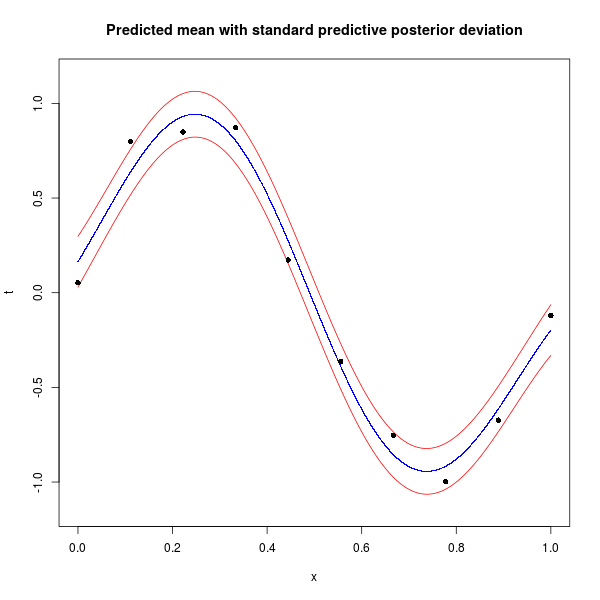
\includegraphics[scale=0.6]{ps2_plot3.png}
\end{center}
\underline{Part 3}. Replicating the plot of the slides:
\begin{center}
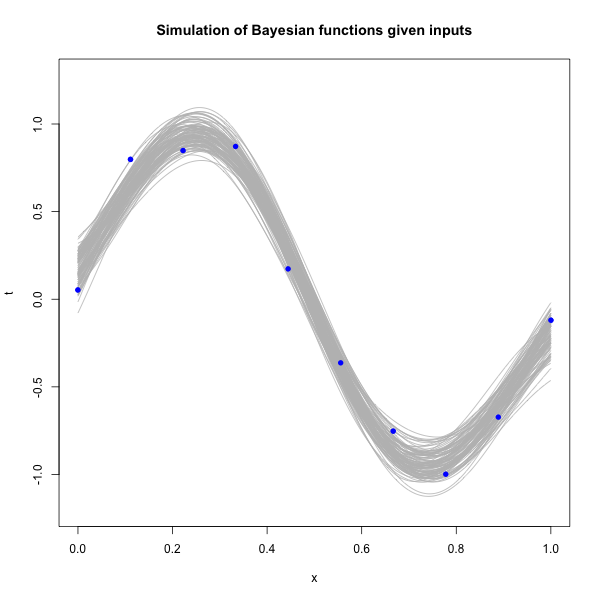
\includegraphics[scale=0.6]{ps2_plot4.png}
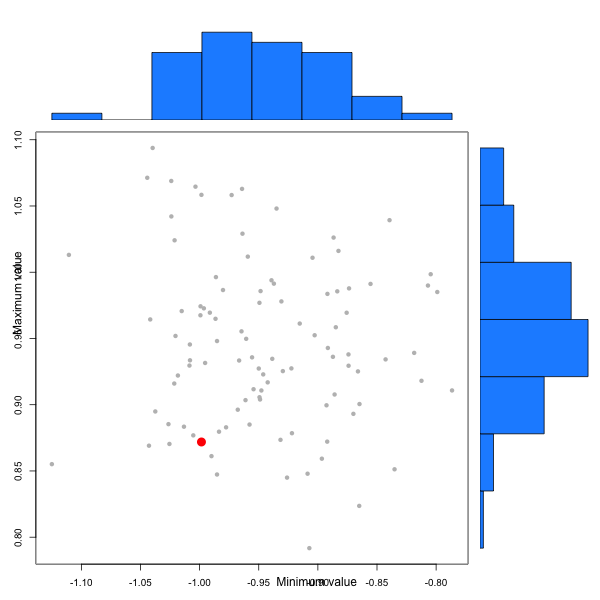
\includegraphics[scale=0.5]{ps2_plot5.png}
\end{center}
% EXERCISE 4
\newpage
\textbf{\underline{Exercise 4}}\\
\newline \underline{Part 1}. \\
\newline We can prove this using the following rule:
\begin{eqnarray}
\phi (\mathbf{x})^T \mathbf{w}_B = \phi (\mathbf{x})^T q \mathbf{Q}^{-1} \phi (\mathbf{x}) \mathbf{t} = \phi (\mathbf{x})^T q \mathbf{Q}^{-1} \sum_{n = 1}^{N} \phi (\mathbf{x}_n) \mathbf{t}_n = \sum_{n=1}^{N} q \phi (\mathbf{x})^T \mathbf{Q}^{-1} \phi(\mathbf{x}_n) t_n  \nonumber
\end{eqnarray}
\newline Where $\mathbf{w}_B$ are the Bayesian parameters. We derive the fact that $\phi (\mathbf{x}) \mathbf{t} = \sum_{n = 1}^{N} \phi (\mathbf{x}_n) \mathbf{t}_n$ by noticing that this product is the inner product between them.\\
\newline \underline{Part 2}. \\
\newline We define:
\begin{eqnarray}
k(\mathbf{x}, \mathbf{y}) = q \phi (\mathbf{x})^T \mathbf{Q}^{-1} \phi (\mathbf{y}) \nonumber
\end{eqnarray}
Then:
\begin{eqnarray}
\phi (\mathbf{x})^T \mathbf{w}_B = \sum_{n=1}^{N} q \phi (\mathbf{x})^T \mathbf{Q}^{-1} \phi(\mathbf{x}_n) t_n = \sum_{n=1}^{N} k(\mathbf{x}, \mathbf{x}_n) t_n \nonumber
\end{eqnarray}
By this definition $k(\mathbf{x}, \mathbf{x}_n)$ becomes the weight of $t_n$ when computing the mean of the predictive distribution $\phi (\mathbf{x})^T \mathbf{w}_B$ at the input location $\mathbf{x}$.\\
\newline \underline{Part 3}. \\
\newline We use the following derivation:
\begin{eqnarray}
\mathbf{K} &=& \left( \begin{array}{ccccc}
k(\mathbf{x}_1, \mathbf{x}_1) & & \cdots & & k(\mathbf{x}_1, \mathbf{x}_K) \\
 & \ddots & & & \\
\vdots & & k(\mathbf{x}_n, \mathbf{x}_k) & & \vdots \\
 & & & \ddots & \\
k(\mathbf{x}_N, \mathbf{x}_1) & & \cdots & & k(\mathbf{x}_N, \mathbf{x}_K) \end{array} \right) \nonumber \\
&=& \left( \begin{array}{ccccc}
q \phi (\mathbf{x}_1)^T \mathbf{Q}^{-1} \phi (\mathbf{x}_1) & & \cdots & & q \phi (\mathbf{x}_1)^T \mathbf{Q}^{-1} \phi (\mathbf{x}_K) \\
 & \ddots & & & \\
\vdots & & q \phi (\mathbf{x}_n)^T \mathbf{Q}^{-1} \phi (\mathbf{x}_k) & & \vdots \\
 & & & \ddots & \\
q \phi (\mathbf{x}_N)^T \mathbf{Q}^{-1} \phi (\mathbf{x}_1) & & \cdots & & q \phi (\mathbf{x}_N)^T \mathbf{Q}^{-1} \phi (\mathbf{x}_K) \end{array} \right) \nonumber \\
&=& q \left( \begin{array}{c}
\phi (\mathbf{x}_1)^T \\
\vdots \\
\phi (\mathbf{x}_N)^T \end{array} \right) \mathbf{Q}^{-1} \left( \begin{array}{c}
\phi (\mathbf{x}_1) \\
\vdots \\
\phi (\mathbf{x}_K) \end{array} \right) \nonumber \\
&=& q \mathbf{\Phi} \mathbf{Q}^{-1} \mathbf{\Phi}^T. \nonumber
\end{eqnarray}
Hence proved.\\
\newline \underline{Part 4}. \\
\newline Given $\lambda = 0$, the proof is the following:
\begin{eqnarray}
\mathbf{K} = q \mathbf{\Phi} (\delta \mathbf{I} + q \mathbf{\Phi}^T \mathbf{\Phi})^{-1} \mathbf{\Phi}^T = \mathbf{\Phi} (\lambda \mathbf{I} + \mathbf{\Phi}^T \mathbf{\Phi})^{-1} \mathbf{\Phi}^T = \mathbf{\Phi} (\mathbf{\Phi}^T \mathbf{\Phi})^{-1} \mathbf{\Phi}^T = \mathbf{H}. \nonumber
\end{eqnarray}

\end{document}
